\documentclass{article}%
\usepackage[T1]{fontenc}%
\usepackage[utf8]{inputenc}%
\usepackage{lmodern}%
\usepackage{textcomp}%
\usepackage{lastpage}%
\usepackage[head=40pt,margin=0.5in,bottom=0.6in]{geometry}%
\usepackage{graphicx}%
%
\title{\textbf{Vecinos en Zulia protestan por bote de aguas negras en el sector Juan Ávila}}%
\author{El Nacional Web}%
\date{03/12/2018}%
%
\begin{document}%
\normalsize%
\maketitle%
\textbf{URL: }%
http://www.el{-}nacional.com/noticias/protestas/vecinos{-}zulia{-}protestan{-}por{-}bote{-}aguas{-}negras{-}sector{-}juan{-}avila\_261924\newline%
%
\textbf{Periodico: }%
EN, %
ID: %
261924, %
Seccion: %
Protestas\newline%
%
\textbf{Palabras Claves: }%
Protestas, Zulia, Denuncia\newline%
%
\textbf{Derecho: }%
2.8%
, Otros Derechos: %
NO\_TIENE%
, Sub Derechos: %
2.8.1%
\newline%
%
\textbf{EP: }%
SI\newline%
\newline%
%
\textbf{\textit{Los habitantes del sector Juana Ávila tienen más de dos años con el problema del servicio de agua}}%
\newline%
\newline%
%
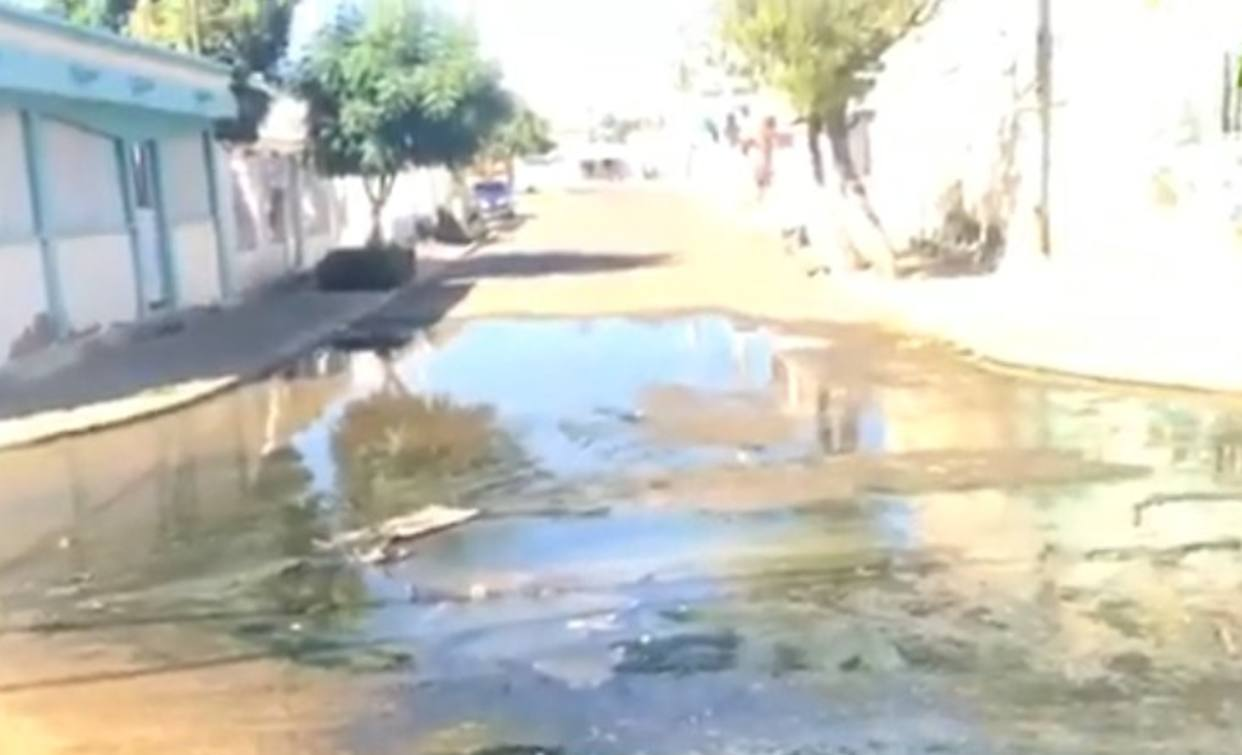
\includegraphics[width=300px]{50.jpg}%
\newline%
%
Vecinos de la comunidad Juana Ávila, en el estado Zulia, protestan~este lunes por el~bote de aguas negras en la zona que no permite el paso por las calles.%
\newline%
%
Los ciudadanos~afirmaron que el problema del servicio de agua en el sector tienen más de dos años en el que no han tenido una respuesta por parte de Hidrozulia.%
\newline%
%
"¿Hasta cuando nos toca vivir así?~Se botan las aguas negras y las aguas blancas vienen con barro, uno~se baña y termina~más sucio", dijo uno de los vecinos de la comunidad.%
\newline%
%
\end{document}